%!TEX root = project.tex

\chapter*{About this project}
\paragraph{Abstract}
This is a basic Action Role Playing Game that allows users to manipulate characters and complete a set of actions including moves and attacks. It has life value calculation system to reflect real-time life value and also allows the character to interact with game objects.\\
This application is designed by Unity 3D, the main program languages are C\# and Java. It allows player manipulates character with the keyboard to control its movement and achieve a set of actions. The Character can be moved by using keyboard "w-a-s-d" to control direction and arrow key "up-down-left-right" can adjust the direction of view.The key "J" is Attack order and key "F" can interact with game objects like communication.\\
This game not only has the player character, it also has monster enemy characters. Monster characters usually patrol on the specific route, once monsters see there is a player character in their detect range, they will catch the player and if the player out of their range, monsters will back to patrol model. This function is an advanced feature, it achieves basic monsters' AI controller.\\
The player character has UI panel to display the information of the character and current situation especially the rest of life value, name, and level of character.\\
\paragraph{Authors}
Qi Fu



\chapter{Introduction}
PC games, also known as computer games or personal computer games, are video games played on a personal computer rather than a dedicated video game console or arcade machine. Their defining characteristics include a more diverse and user determined gaming hardware and software, and a generally greater capacity input, processing, and video output.

Home computer games became popular following the video game crash of 1983 leading to the era of the "bedroom coder". In the 1990s, PC games lost mass-market traction to console games before enjoying a resurgence in the mid-2000s through digital distribution.

Newzoo, reports that the PC gaming sector is the third largest (and estimated in decline), with the consoles second largest, and across all platforms as of 2016, 2.2 billion gamers generate US\$101.1 billion in revenue (i.e. all numbers exclude hardware costs), and "Digital game revenues will account for \$94.4 billion or 87\% of the global market. Mobile is the most lucrative segment, with smartphone and tablet gaming growing 19\% year on year to \$46.1 billion, claiming 42\% of the market. In 2020, mobile gaming will represent just more than half of the total games market. China expected to generate \$27.5 billion, or one-quarter of all revenues in 2017." PC is considered synonymous (by them and others) with IBM PC compatible systems; while mobile computers – smartphones and tablets, such as those running Android or iOS – are also personal computers in the general sense. The "APAC" region is estimated to generate \$46.6 billion in 2016 or 47\% of total global game revenues (note, not only "PC" games). China alone accounts for half of APAC's revenues, reaching \$24.4 billion, cementing its place as the largest games market in the world, ahead of the US's anticipated market size of \$23.5 billion. China is expected to have 53\% of revenues from mobile in 2017 (46\% in 2016). The uncoordinated nature of the PC game market and its lack of physical media make precisely assessing its size difficult.\cite{einstein}\\
Types of Game\\
RPG: Role-playing Game is a game in which players assume the roles of characters in a fictional setting. Players take responsibility for acting out these roles within a narrative, either through literal acting or through a process of structured decision-making or character development. Actions taken within many games succeed or fail according to a formal system of rules and guidelines.

WEG: Web Game(Browser Game) is a computer game that is played over the Internet using a web browser. Browser games can be run using standard web technologies or browser plug-ins. The creation of such games usually involves the use of standard web technologies as a frontend and other technologies to provide a backend. Browser games include all video game genres and can be single-player or multiple-player. Browser games are also portable and can be played on multiple different devices, web browsers, and operating systems.

ACT: Action Game is a video game genre that emphasizes physical challenges, including hand-eye coordination and reaction time. The genre includes diverse subgenres such as fighting games, shooter games and platform games which are widely considered the most important action games, though multiple-player online battle arena and some real-time strategy games are also considered to be action games. In an action game, the player typically controls the protagonist or avatar. The avatar must navigate a level, collecting objects, avoiding obstacles, and battling enemies with various attacks. At the end of a level or group of levels, the player must often defeat a boss enemy that is more challenging and often larger than other enemies. Enemy attacks and obstacles deplete the avatar's health and lives, and the player receives a Game over when they run out of lives. Alternatively, the player wins the game by finishing a sequence of levels. But some action games, usually arcade games, are unbeatable and have an indefinite number of levels; and the player's only goal is to maximize their score by collecting objects and defeating enemies.

\chapter{Context}
GitHub Link: \href{https://github.com/QiFuChina/RPG}{github.com/QiFuChina/RPG}. 
It contains:
\begin{itemize}
\item Application package.
\item Documents of application. 
\item Assets Package.
\item Source codes of application.
\end{itemize}
Video Line: \href{https://youtu.be/4Db_27HFujA}{here}
\section{Application Information}
\begin{itemize}
\item Design Platform
:
Windows Computer
\\
\item Design Technology
:
Unity 3D
\\
\item Design Model
:
Single client service
\\
\item Game Type
:
Role-Playing Game
\\
\item Design Inspiration
:
It is from a Chinese Wuxia online game.
\\
\item Manipulate
:
The Character can be moved by pressing keyboard "w-a-s-d" to control the direction, "up-down-left-right" can adjust the direction of view.The key "J" is attack order and key "F" can interact with game objects like communication.
\\
\item Model
:
The character model relative with animations, the player press keyboard then the model will reflect a set of animation as feedback
\\
\item Objects
:
The enemy has "enemy" target that different with the character when enemies closed to the character it will attack the character.
\end{itemize}

\subsection{Expected Objectives}
{\textbf{Basic Objectives:}}

\begin{itemize}
\item Completely moving functions and player character status display scripts.

\item Attack and hurt function.

\item Monster enemies controller.
\end{itemize}
{\textbf{Advanced Objectives:}}
\begin{itemize}
\item Game data save and load.

\item Monsters AI tree.

\item Animation controller.

\item Player inventory system.
\end{itemize}


\chapter{Methodology}

\begin{itemize}
\item Agile / incremental and iterative approach to development. \\
This project aimed at basic functions of the regular role-playing game at first, and then develop the advanced functions after basic functions are finished. 
\item What about validation and testing? \\
It can be worked successfully in the windows 10 64bit system. 
\item If team based, did you use GitHub during the development process.\\
No, this is an individual project, but I am looking forward using GitHub during team development process.
\item Selection criteria for algorithms, languages, platforms, and technologies.\\
C\# is the wide language that is used in Unity 3D game development industry so that is the reason why I used C\# and Unity 3D to develop this project.
\end{itemize}


\chapter{Technology Review}
\section{Scripts of Game Objects}
\begin{itemize}
This graph is the structure of the application, Unity is the design platform and it contains C\# scripts and animation controller. The command will be input from keyboard and application will process it to present in the game world.\\
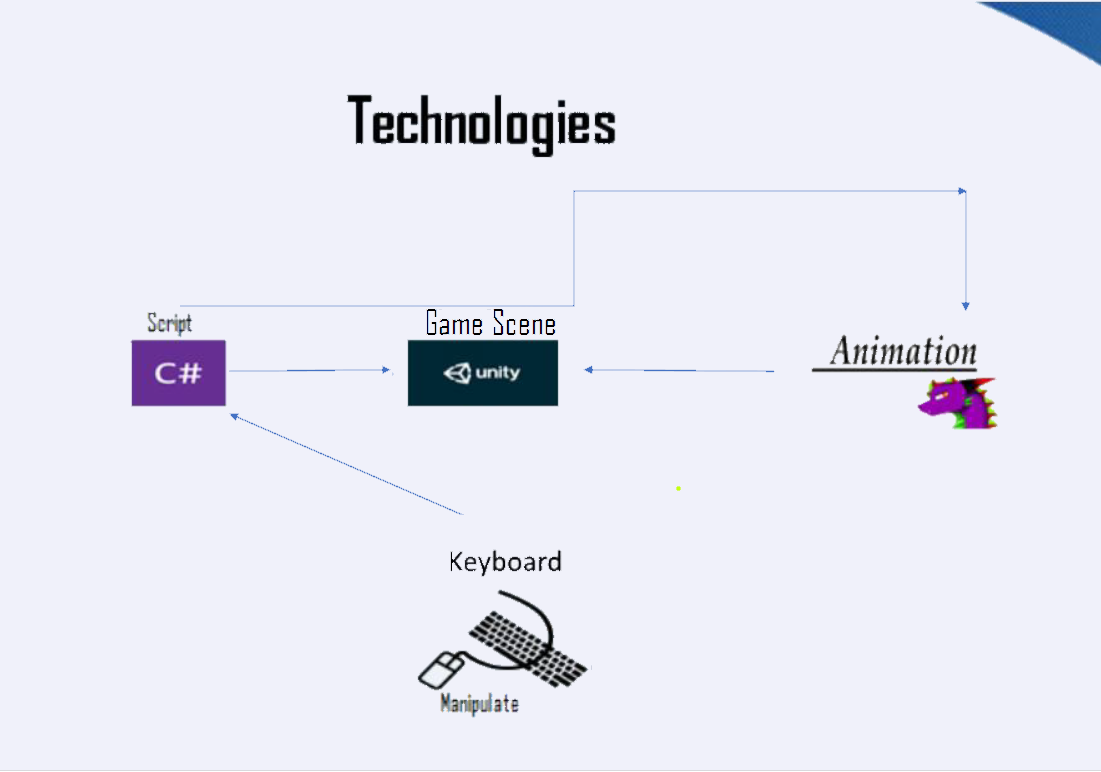
\includegraphics[scale=0.5]{img/MainGraph.png}\\
Description :\\
\item Unity is a cross-platform game engine developed by Unity Technologies\href{https://venturebeat.com/2014/10/23/john-riccitiello-sets-out-to-identify-the-engine-of-growth-for-unity-technologies-interview/}{[2]}, which is primarily used to develop both three-dimensional and two-dimensional video games and simulations for computers, consoles, and mobile devices. First announced only for OS X at Apple's Worldwide Developers Conference in 2005, it has since been extended to target 27 platforms\href{https://unity3d.com/cn/unity/features/multiplatform}{[3]}\href{https://insights.dice.com/2013/06/03/how-unity3d-become-a-game-development-beast/}{[4]}. Six major versions of Unity have been released. For a list of games made with Unity, visit List of Unity games.\\
Unity is a multipurpose game engine that supports 2D and 3D graphics, drag-and-drop functionality and scripting using C#. Two other programming languages were supported: Boo, which was deprecated with the release of Unity 5\href{https://unity3d.com/cn/unity/whats-new/unity-5.0}{[5]} and JavaScript which started its deprecation process in August 2017 after the release of Unity 2017.1\href{https://blogs.unity3d.com/cn/2017/08/11/unityscripts-long-ride-off-into-the-sunset/}{[6]}.

The engine targets the following graphics APIs: Direct3D on Windows and Xbox One; OpenGL on Linux, macOS, and Windows; OpenGL ES on Android and iOS; WebGL on the web; and proprietary APIs on the video game consoles. Additionally, Unity supports the low-level APIs Metal on iOS and macOS and Vulkan on Android, Linux, and Windows, as well as Direct3D 12 on Windows and Xbox One.

Within 2D games, Unity allows importation of sprites and an advanced 2D world renderer. For 3D games, Unity allows specification of texture compression, mipmaps, and resolution settings for each platform that the game engine supports,\href{https://unity3d.com/cn/unity/features/multiplatform}{[3]} and provides support for bump mapping, reflection mapping, parallax mapping, screen space ambient occlusion (SSAO), dynamic shadows using shadow maps, render-to-texture and full-screen post-processing effects\href{https://web.archive.org/web/20130312140345/http://docs.unity3d.com/Documentation/Manual/DirectX11.html}{7}. Unity also offers services to developers, these are: Unity Ads, Unity Analytics, Unity Certification, Unity Cloud Build, Unity Everyplay, Unity IAP, Unity Multiplayer, Unity Performance Reporting and Unity Collaborate.


\item Completely moving functions and player character status display scripts.
\\
Here is the technology of character moving functions:\\
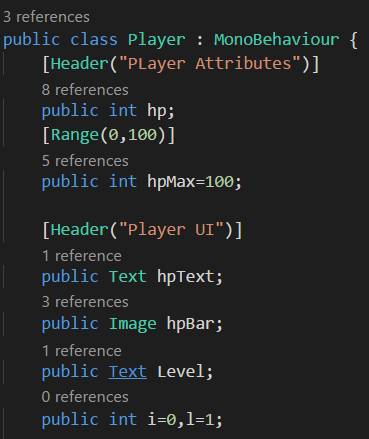
\includegraphics[scale=0.5]{img/Attributes1.png}
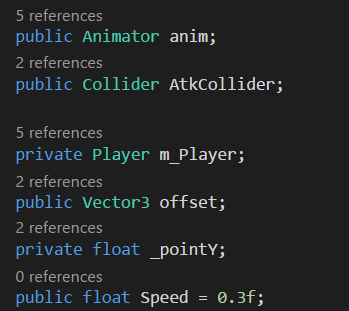
\includegraphics[scale=0.5]{img/Attributes2.png}\\
These variables are player character attributes\\

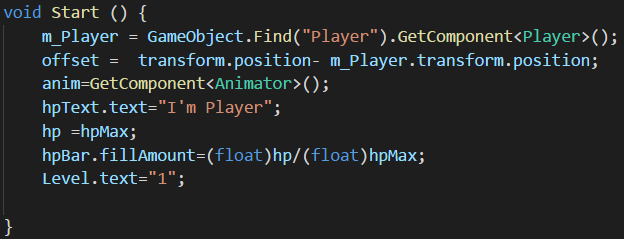
\includegraphics[scale=0.5]{img/Character.png}\\{Figure 1}\\
After game sense be loaded, the start function will be executed first to find the game object that name is "Player" and access its position, then set the default name, healthy value, and level to the character.\\

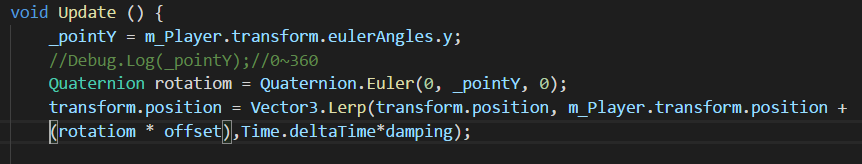
\includegraphics[scale=0.4]{img/Camera.png}\\{Figure 2}\\
The update function will be updated every frame to detect the player character status and the first thing is making the camera look at the character in the fixed degree.\\


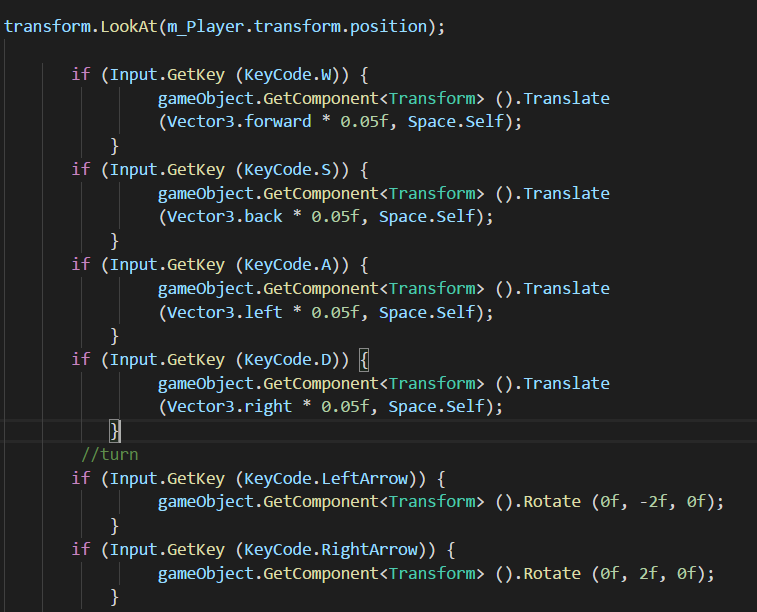
\includegraphics[scale=0.4]{img/Moving.png}\\{Figure 3}\\
After camera look at the player, the update function will be called each frame, once player input commands through the keyboard, the relative function will be executed.\\
From this picture, we know "w-s-a-d" and "←-→" keys allow the character to move.\\

\item Attack and hurt function.
\\

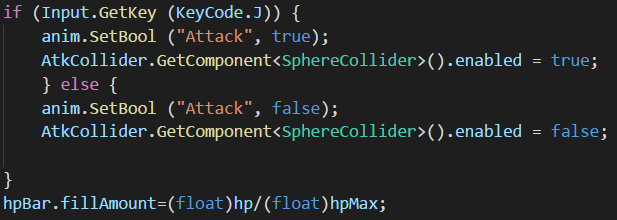
\includegraphics[scale=0.4]{img/Attack.png}\\{Figure 4}\\
The key "J" is the attack command that links the animator controller and object collider which connect with the player character. If "J" be triggered, the animation of "Attack" will play and the atksphere collider will enable to be detected.\\
The hp expression make sure the healthy value keeps updating all the time.\\

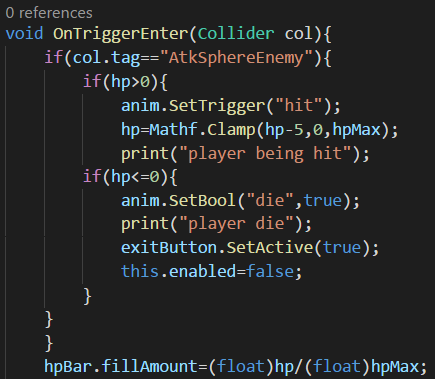
\includegraphics[scale=0.5]{img/AttackTrigger.png}\\{Figure 5}\\
This function relative to object collider, when player attack collider collides with the specific collider, the result will trigger animator controller and update the healthy value.

\item Monster enemies controller.
\\

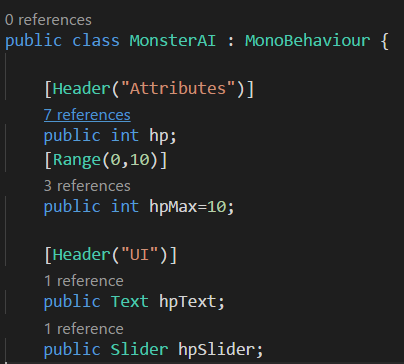
\includegraphics[scale=0.5]{img/MonsterAttributes1.png}
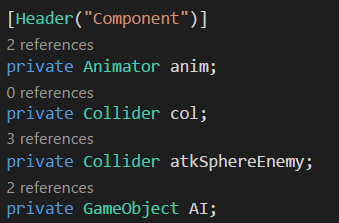
\includegraphics[scale=0.5]{img/MonsterAttributes2.png}\\
These variables are monsters attributes.\\

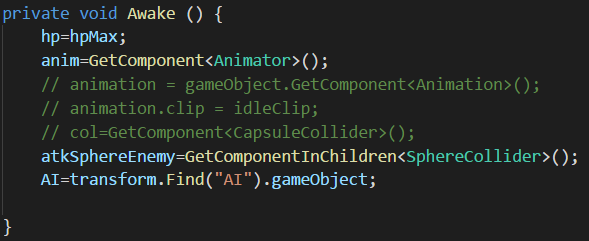
\includegraphics[scale=0.5]{img/AI.png}\\{Figure 6}\\
The awake function will execute when program initialized. It will awake the game component "AI" that binding with monster objects.\\

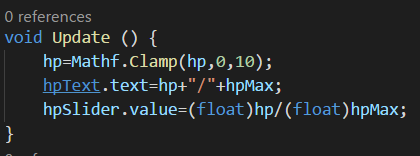
\includegraphics[scale=0.5]{img/MonsterLP.png}\\{Figure 7}\\
Initialized monsters healthy value every frame and response to monsters canvas.\\

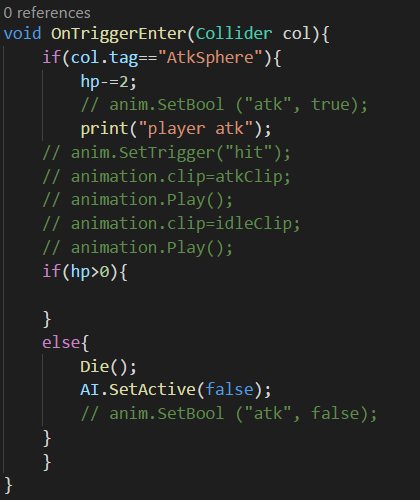
\includegraphics[scale=0.5]{img/MonsterTrigger1.png}
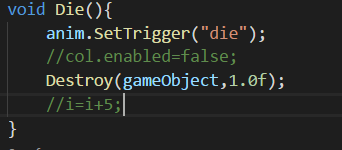
\includegraphics[scale=0.5]{img/MonsterTrigger2.png}\\
Once the trigger function detects monsters collide with other objects which target is "AtkSphere",  monsters healthy will be decreased. When the healthy value under 0, the object will be destroyed.\\

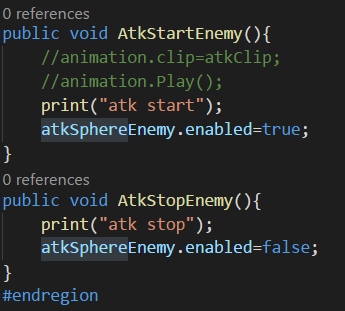
\includegraphics[scale=0.5]{img/MonsterAtk.png}\\{Figure 8}\\
This function is attack function, when monsters collide with character then attack function will call attack animator and enable the sphere collider to make game update monsters and player healthy value.
\end{itemize}

\section{Monsters AI}
This is a tool of monsters AI controller.
\\
\begin{itemize}
\item After downloading the RAIN package, import it and open it on the Unity edit row, selecting one object and click RAIN→Create New→AI to add the AI component to the target object.  \\
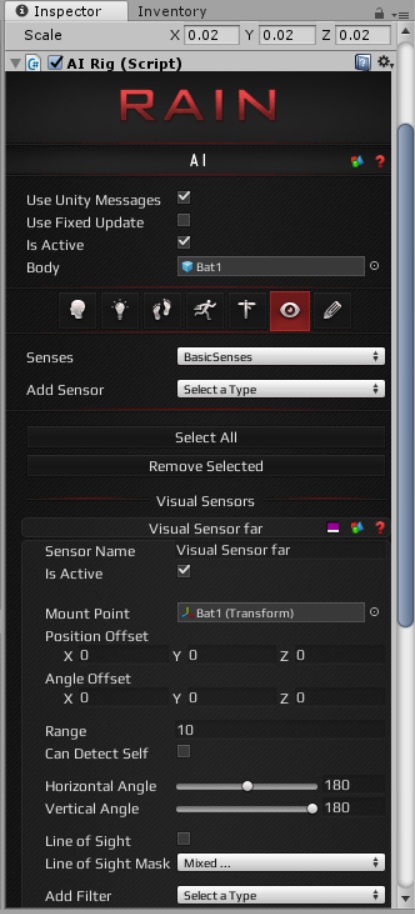
\includegraphics[scale=0.5]{img/RainInspector.png}\\
\item This component has two visual sensors: far and near. These sensors make monsters can "see" the player character if they are closed.\\
\item The AI tree sets a list of condition to make monsters can execute correct performance under different situations.\\
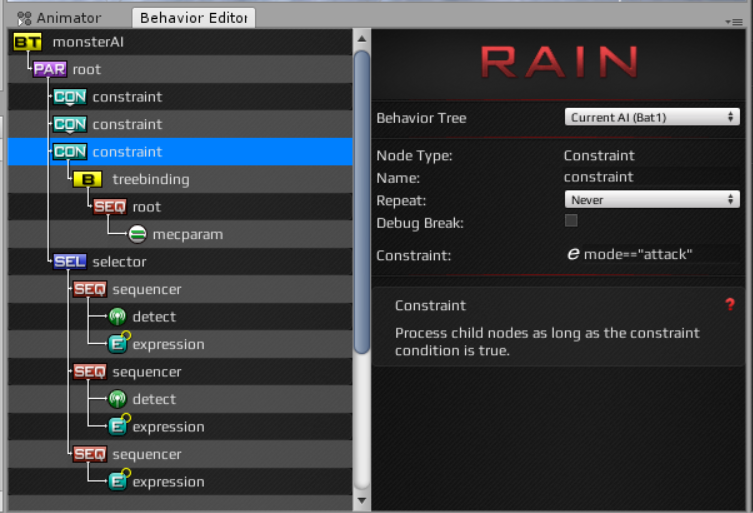
\includegraphics[scale=0.5]{img/RainWindows.png}
The constraint command is conditional judgment statement. To set a key value of the condition previously and create "waypointpatrol", once condition was triggered then relative constraint commands will be executed. And the same level of constraints are parallel relationship it means one constraint can break another constraint.\\
\item This is selector command.\\
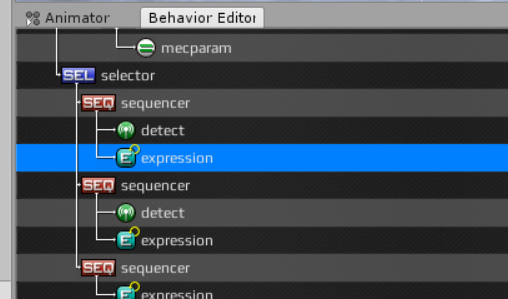
\includegraphics[scale=0.5]{img/RainSelectE.png}\\
The selector will select one sub sequencer when the triggered condition be executed.\\
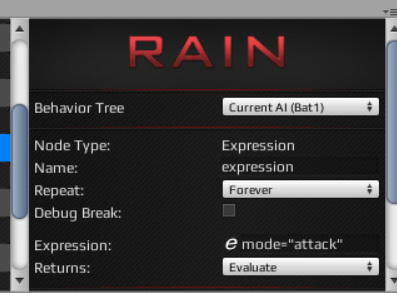
\includegraphics[scale=0.5]{img/RainSelect.png}\\
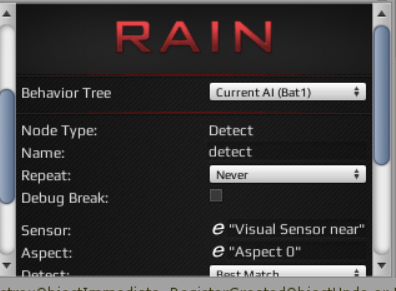
\includegraphics[scale=0.5]{img/RainSelectD.png}\\
It is an example of attack command, we can see when the near of visual sensor detect the player character, the expression value will become attack that means the animator will be called, then it will call animation to play attack function and atksphere will enable to calculate the damage.
\end{itemize}

\section{Inventory System}
This is a tool of character inventory system.
\begin{itemize}
\item After download the Inventory System package, import it and open it on the Unity edit row, selecting one object and click Windows→Inventory to add the Inventory System component with the target object and just click suit it up.\\
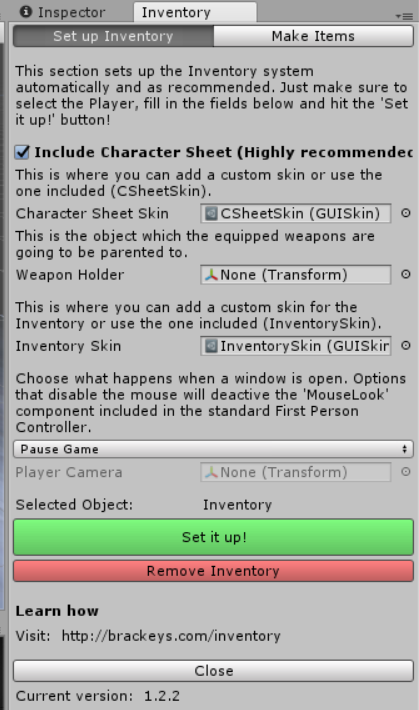
\includegraphics[scale=0.5]{img/ISI.png}\\
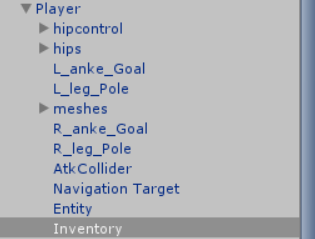
\includegraphics[scale=0.5]{img/ISP.png}\\
After that, select a weapon object and add components "Rigidbody", "BoxCollider", "Item" and "First Person Pick Up" scripts. In the weapon object, changing these attributes to make weapon can be picked.\\
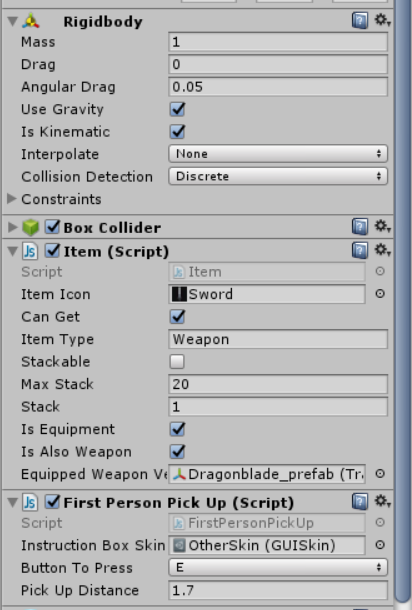
\includegraphics[scale=0.5]{img/Weapon.png}\\
\end{itemize}



\section{Data}
\begin{itemize}
These scripts manage the game data function.\\
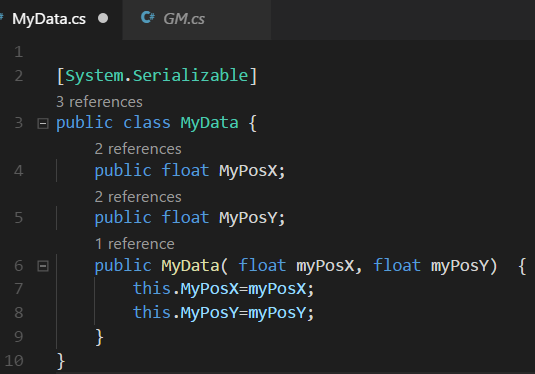
\includegraphics[scale=0.5]{img/Data.png}\\
The Data.cs file created a class to store the position of the player character.\\
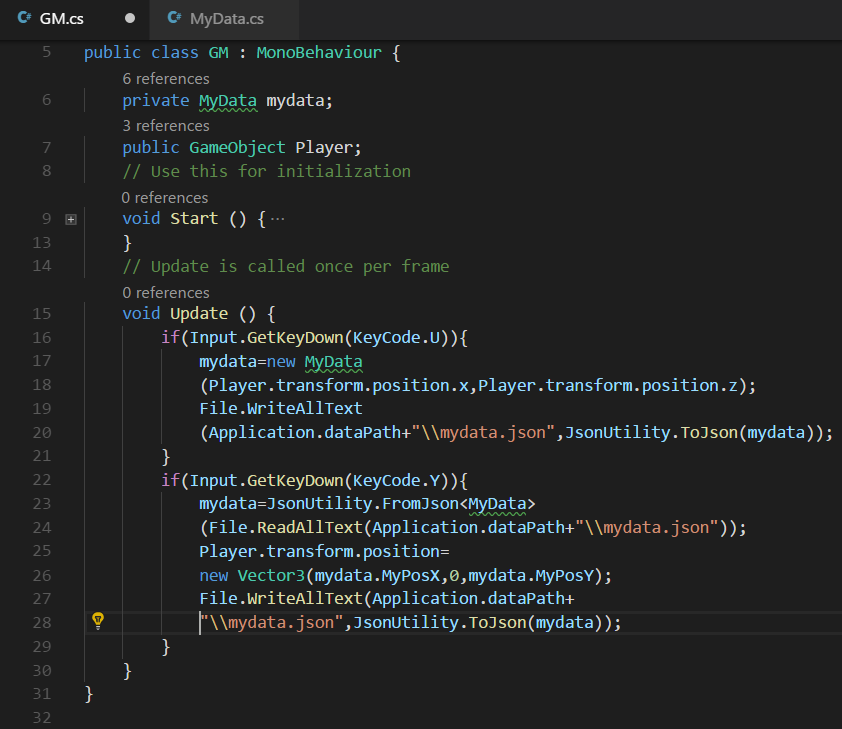
\includegraphics[scale=0.4]{img/GM.png}\\
This GM.cs file used the function that in the Data.cs and defined a variable to get the player character.\\
Functions which inside in update are saved and loaded commands, users press "U" to get current position and "Y" to rewrite the player position.\\
The expression \\
"\emph{mydata=new MyData(Player.transform.position.x,Player.transform.position.z);}" will get position and save them to the variable mydata as Jason format.\\
The expression \\
"\emph{File.WriteAllText(Application.dataPath+"//mydata.json",JsonUtility.ToJson(mydata));}" will acquire the player position when press "Y", and change data format from Jason to transform position then save it in the local directory, then apply them to the game object.
\end{itemize}

\chapter{System Design}
The architecture of player character\\
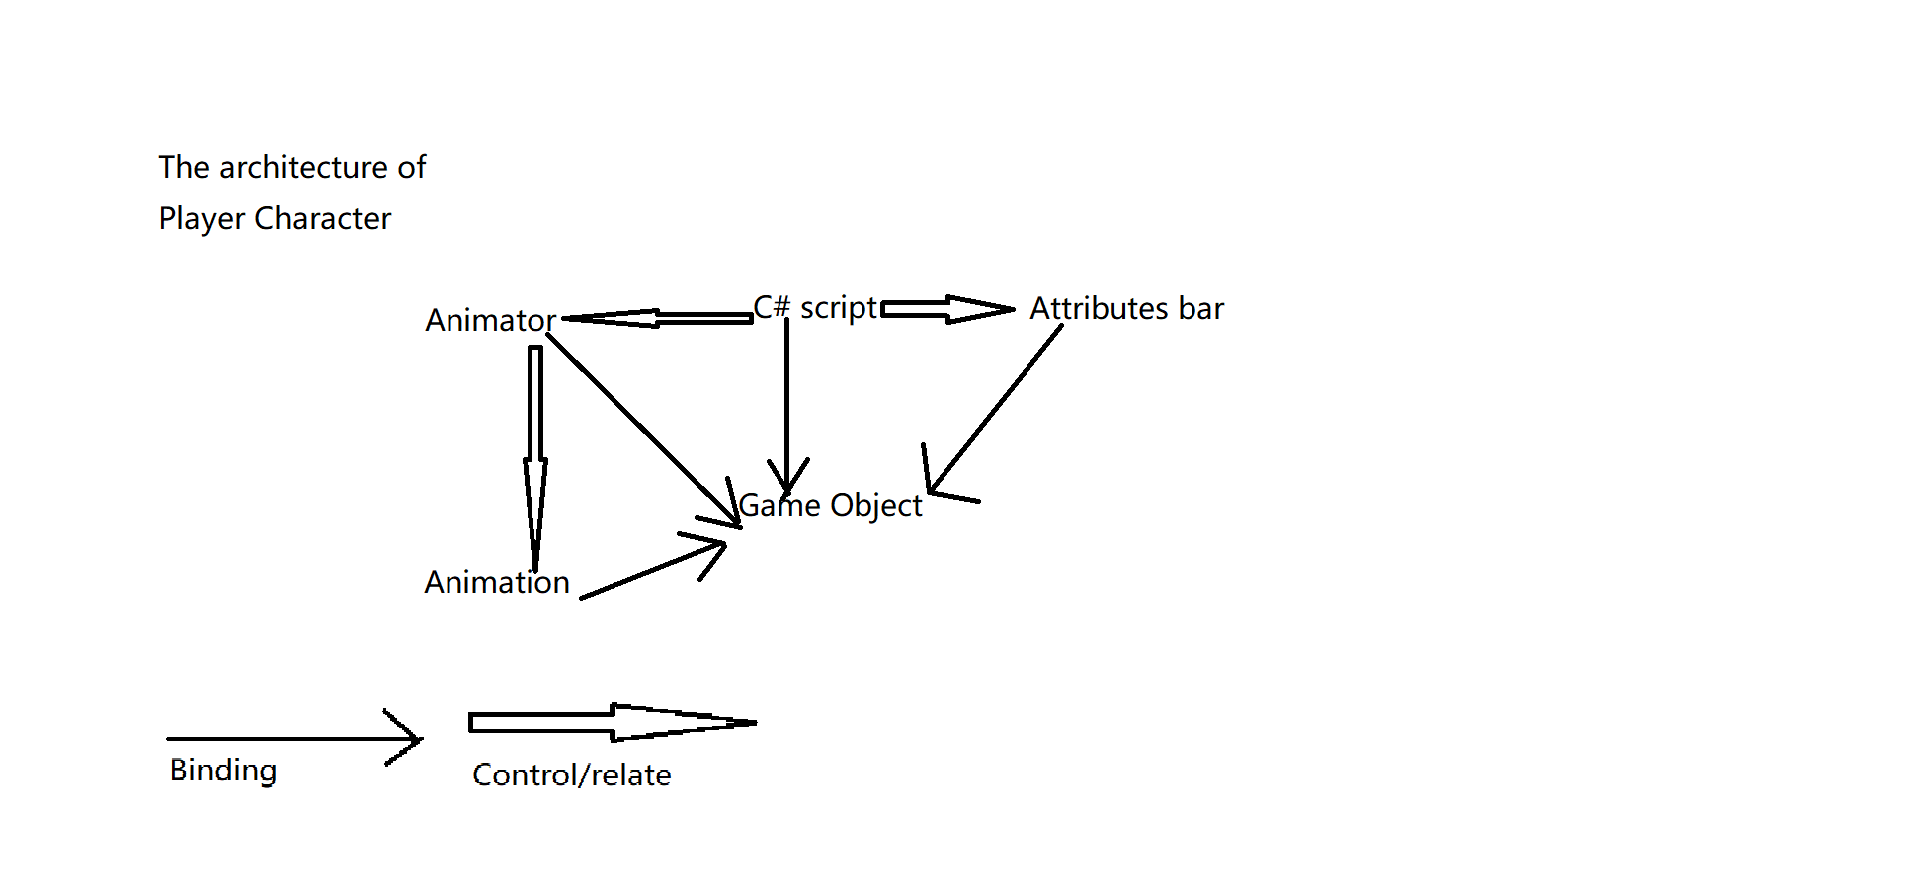
\includegraphics[scale=0.5]{img/ArchitectureOfPlayer.png}\\
From the above picture, we know the player game object bindings with the rest of components and components also have relationships with themselves, results that will be generated from components will transfer to game object finally.    
\begin{itemize}
\item C\# scripts, animator, and animation have the control relationship. When users manipulate the character through the keyboard, C\# scripts will send commands to animator, after the animator receives commands it will call the animation component, then the animation component will call relative actions and transfer them to a game object.\\
\item There is another condition that is the character be triggered by other game objects in the game, then the C\# script also will call the animator to continue events. \\
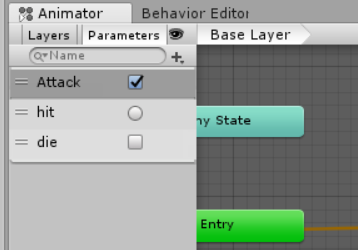
\includegraphics[scale=0.5]{img/PlayerP.png}\\
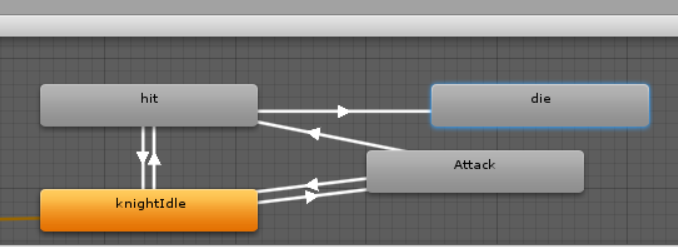
\includegraphics[scale=0.5]{img/PlayerA.png}\\
\end{itemize}


The architecture of monsters\\
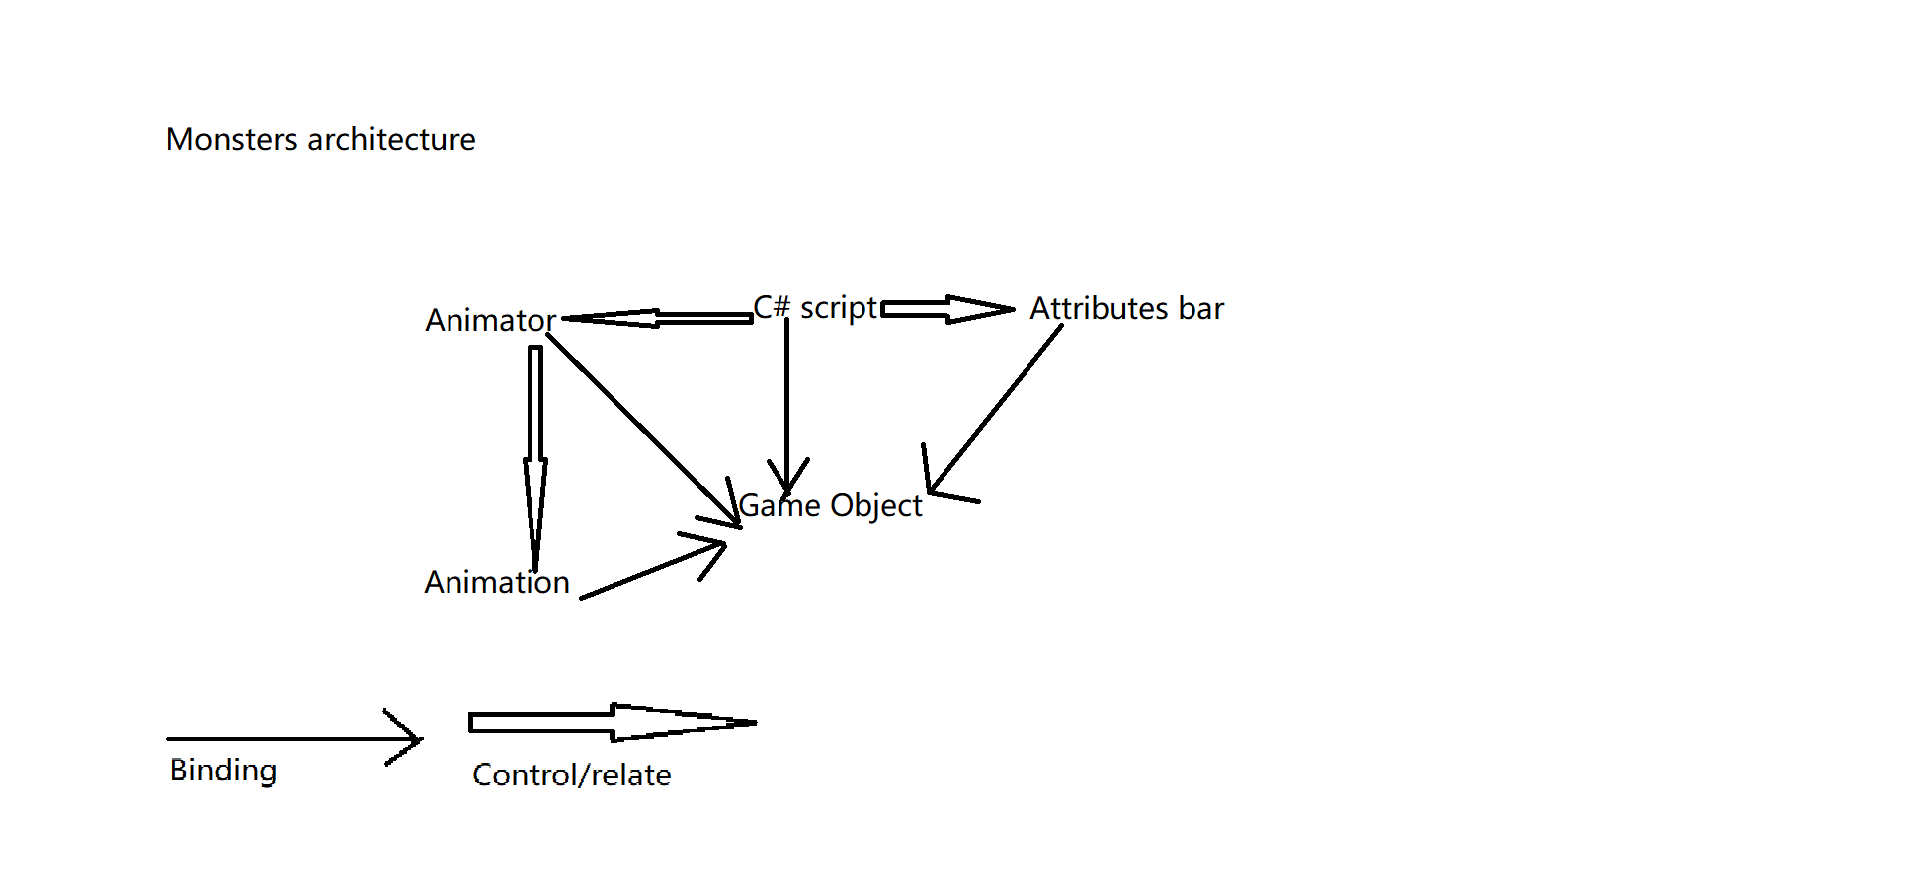
\includegraphics[scale=0.5]{img/ArchitectureOfMonster.png}\\
The monster relationships are similarly with the player character.
The animator controller in the below:\\
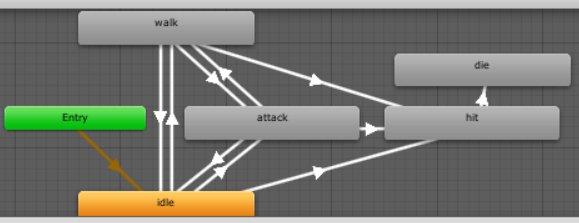
\includegraphics[scale=0.5]{img/MonsterAinmator.png}\\
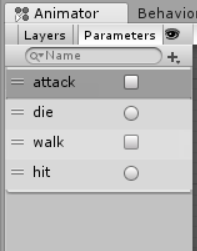
\includegraphics[scale=0.5]{img/MonsterP.png}\\
\item From these above pictures, we know each animation status enable to trigger another and break current status. The white arrow is a transition to change their status with the artificial operation.
\item These animators can be awakened by C\# scripts to achieve animation status changing.

\chapter{System Evaluation}
Size of application
\begin{itemize}
\item This game total size is 167M with 64-bit and 162M with 32-bit. The evaluation device information in the below.\\

\\
The 64-bit application occupies about 28\% CPU, 95MB of memory, and about 60\% GPU when it runs. The 32-bit application has the similar consumption. 
\item From the above result, we can see the performance benchmarks of application is not good enough because it consumes excessive resource as a basic role-playing game.
\end{itemize}
The outcomes of application
\begin{itemize}
\item From the introduction, there are 7 objectives to work and now, the basic objectives almost finished except some functions can be built more perfect. The advanced objectives of Monster AI tree and animation controller all almost finished. The inventory system is successful to acquire weapons but cannot make the player get extra enhance effects. The game save and load function can read and save player position as Jason file then load it but not able to record all information about the player.
\end{itemize}
limitations
\begin{itemize}
\item The first limitation of the application is users cannot rotate the character view direction by moving the mouse. It is obvious that moving the mouse to change view better than press "←→" keys.
\item Another limitation is the inventory system, this is an asset package that was designed by another developer. I only worked the small part of the entire system that I understood. 
\end{itemize}

\chapter{Conclusion}
Overall
\begin{itemize}
\item To review the whole context, the aim of the application is to build a role-playing game that has complete basic functions to play and has some advanced functions to improve users experience. And basic functions are finished mostly, advanced functions still have some part need to complete.
\end{itemize}
The outcomes of the project
\begin{itemize}
\item The Keyboard can manipulate the player character.
\item The character can play exist animation when relative commands are triggered. For example, the character can play attack animation when pressing "J".
\item Monsters are able to play animation when they attacked.
\item The value of healthy will update automatically. 
\item The character and monsters can attack each other when life value becomes 0, it will die and the game object will be destroyed from the screen. 
\item Monsters will obey the AI tree system to perform. 
\item The player character can pick a weapon from the ground and open bags to catch it.
\item The save function can read the position and load it.
\end{itemize}
summary
\begin{itemize}
This game just meets regular functions, some advanced functions like equipment effect, high intelligent enemies and more functions that exist in publish role-playing game are not created. A single play game should have full save and load functions, it can be saved in the local directory or cloud service either. 
Obviously, this application can become a game that has various functions and I am enjoying the experience of working this game.
\end{itemize}